\documentclass[11pt]{article}
\usepackage{colacl}
\usepackage{graphicx}
\sloppy



\title{COMP30027 Machine Learning - Project 2 Report}
\author
{Anonymous}

\begin{document}
\maketitle

%\begin{abstract}
%Don't include an abstract.
%\end{abstract}

\section{Introduction}

This project aims to predict the geolocation of tweet users only based on tweet text among four cities, which are Melbourne, Sydney, Perth and Brisbane. Two systems are designed for classification, they are WLH-based system and WLH with Word2Vec based system.

\section{Related Literature}

Following the efforts made by K.Pappas et al.[1], the Word Locality Heuristic(WLH) proposed  by them is adopted. WLH could help identify locality words for city. WLH is a statistic that assign the words highly used in specific place with a high value, while words distributed evenly across different states with low value.
\newline\newline
Below is the WLH formula, w, s, S represent a word, a city, all cities respectively.\\

{\centerline {\textbf{\textit{WLH(w) = $\max_{s \in \mathcal{S}}$ $\frac{P(w|s)}{P(w)}$}}}}

\section{Feature Engineering}
Each tweet is a natural language short text, so \textbf{ the bag of words model} is the most suitable \textbf{data representation} to capture information about each tweet, which represents the information in a continuous format. 
\newline\newline
There are more than 100,000 words in the training dataset, it is impossible to include all of them in the model and train them on a regular computer, so\textbf{ feature selection} is vital. Strings like\textbf{ ULRs, unicodes and punctuations} are removed before feature selection. Because they are useless for tweet location prediction and would provide noise information. For example, if not remove url, words like u and uu would be included in the bag of words model. Furthermore,\textbf{ the common English word}, such as "a", "the" and so on, are removed to increase the efficiency of training, since they are commonly used and not representative.\\\\
In this project, there are\textbf{ two main criterions} of qualifying word, a word's WLH value and frequency of a word. The reasons support these two criterions would be discussed in following sections.\\\\
Firstly, the rationale behind choosing\textbf{ words with high WLH} is based on the paper by K.Pappas et al.[1]. A word with high WLH means that it could give valuable information about location. Conversely, a word with low WLH means that it is commonly used across several cities, which provide less information about location. Thus, words with high WLH are more preferable in this project.\\\\
Secondly, the frequency of a word is essential. Because a word that appears only 1 or 2 times could have a high WLH value, but it is very unlikely to appear in the development dataset, so it provides almost no information about the location of a tweet. To address this issue, word that beyond a pre-defined\textbf{ frequency threshold} could increase the probability that a word appear in another tweet again. In addition, in this project, 15 is found to be the most suitable frequency threshold.\\\\\
Finally, words occurred more than 15 times and with top 630 WLH in each city are selected into the bag of words model. Due to the constraint of RAM , 630 is the max number of features for each city that my personal computer could implement.
\section{Learner selection} 
Different learner is good at different tasks, so the choice of learner is important. In this project, logistic regression, Naïve Bayes and KNN classifiers  are considered.\\
\subsection{Hyperparameter Tuning}
Hyperparameter is a constant defined before the training of a classifier, it has influence on the performance of a classifier.\\\\
For the Naïve Bayes classifier, multinomial Naïve Bayes is selected, since the data representation is a vector of word counts. This means that there are multiple categories of words and this follows the definition of the multinomial distribution.\\\\
For the KNN classifier, the cosine distance similarity is considered due to the high sparsity of the training data. Two tweets have closer cosine value are more similar. Then, 3 is selected to be k, because odd number could avoid the tie situation and 5 is too slow to train, so, 3 is more preferable.
\section{Evaluation}
In this section, two systems the WLH-based system and the WLH-and-Word2Vec based system would be evaluated in order.
\subsection{WLH-based system}
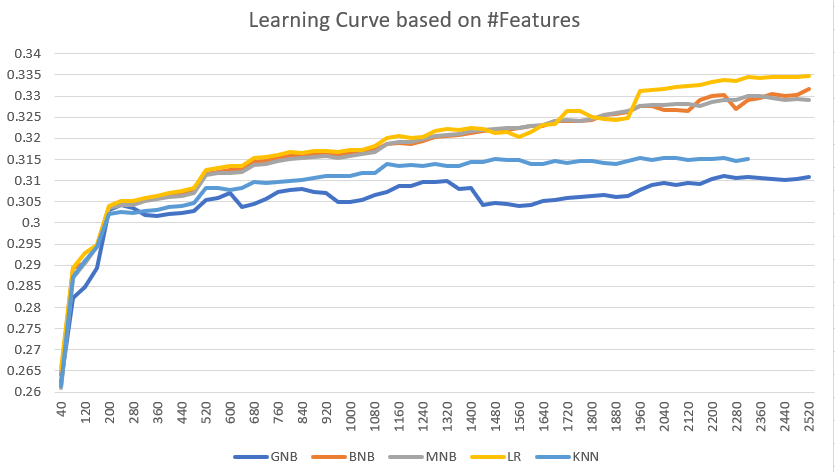
\includegraphics[scale=0.48 	]{learningCurve}
The WLH-based system trains logistic regression, MNB, GNB, BNB, and KNN classifier on the features selected based on the two criterions discussed above.
\subsubsection{Behaviour of the methods}
From the learning curve (on the bottom-left corner of this page) obtained from the development dataset, there are mainly three things can be shown. \\\\
Firstly, logistic regression has the best accuracy performance of around 33.5\% among all single classifiers, because the training data is continuous and logistic regression classifier is good at this. \\\\
Then, among the family of Naïve Bayes classifiers, both GNB and MNB perform better than GNB, this follows what has been discussed in the hyperparameter tuning section, which claims that the distribution of word frequency is not binomial. \\\\
By the way, KNN classifier consume most memory among all classifiers, thus, the max number of feature for each city is 580.\\\\
Finally, there is a almost a positive relationship between number of features and accuracy of classifiers, thus accuracy could be increased by adding more features.
\subsubsection{Error analysis}
Firstly, after checking the training dataset, more than 50\% of training instances contains all zero, which makes prediction very hard.\\\\
 Secondly, there is a problem of overfitting. By searching those selected \#event and username in the development dataset, most of those \#event and username do not appear in the development dataset again. This means they are not presentative and do not provide the information expected by its WLH value. The reason behind this may due to that if an event past, people are less likely to mention it again. Based on this, \#event and username are removed before selection.\\
\includegraphics[scale= 0.75]{confusionMatrix}\\
The table above is the confusion matrix constructed by the logistic regression classifier on the development dataset. It shows that most of tweets are classified as Perth, which leads to a lot of mistakes. The reason behind this behaviour is that there are over 50\% instances with all 0, and the classifier predict all of them as Perth.\\
\subsection{WLH-and-Word2Vec based system}
To address the issue of over 50\% instances are all zero, this WLH-and-Word2Vec based system is designed. Short text tweet is the main cause of this issue, it does not provide enough information on frequency. But, how about the context? In this system, the value of each entry of an instance is not frequency. Instead, for each entry, its value is the sum of the top 3 Word2Vec similarity to the corresponding selected word.\\
\subsubsection{Behaviour of the methods} 
The result of this system shows that the percentage of all zero instances reduce significantly, there are only 6\% of instances are all zero. However, this technique does not help classifier to give a better performance, instead, each learner gives only 25\% accuracy on the development dataset.
\subsubsection{Error analysis}
Word2Vec is a technique which assign vector to each word depends on its context, but it is not suitable in this task. For instance, for the word melbourne, the two words with top 2 similarity are sydney and perth, since they all represent a place and have similar context. This is would add misleading information, because Melbourne citizens tend to use melbourne while Sydney citizens tend to use sydney, which means they should not be similar in this task. Thus, classifiers behave badly in this system.

\section{Conclusions}

In conclusion, bag of words model is used as the data representation. And the value of WLH as well as the frequency of a word are the two main criterions used to select features in this project. In addition, URLs, unicodes, mentions, hash tags, common English words and punctuations are removed before feature selection. Then, WLH-based system and WLH with Word2Vec based system are designed for classification. From the learning curve, logistic regression is the best classifier, Gaussian Naïve Bayes is not suitable for this task and there is a positive relationship between accuracy and number of features. In addition, the shortage of information due to short text is the biggest challenge for achieving a good accuracy.

\bibliographystyle{acl}
\begin{thebibliography}{2018}
	\bibitem{[PapAzaMih18}
	[1] K.Pappas, M.Azab and R.Mihalcea,
	\emph{A Comparative Analysis of Content-based Geolocation in Blogs and Tweets}.
	
\end{thebibliography}
\end{document}
